The Standard Model (SM) of particle physics is the theoretical framework that describes the interaction of matter through the strong, electromagnetic, and weak forces.
Figure \ref{Theory:SM} shows the bosons and fermions in the SM.
The matter particles are represented in three generations of fermions, with particles in each generation being heavier than the previous. 
The electromagnetic force is mediated by the photon, which interacts with charged particles.
The weak force in mediated by the W and Z bosons.
The strong force describes the interactions between quarks and gluons, and is mediated by the gluon.
Finally, there is also the Higgs boson, which is the remnant of the Higgs field that was introduced to give mass to the bosons and fermions.
The strong force is described by QCD.
This thesis is concerned with QCD measurements, and more detail about QCD is given in this chapter.


\begin{figure}
\centering
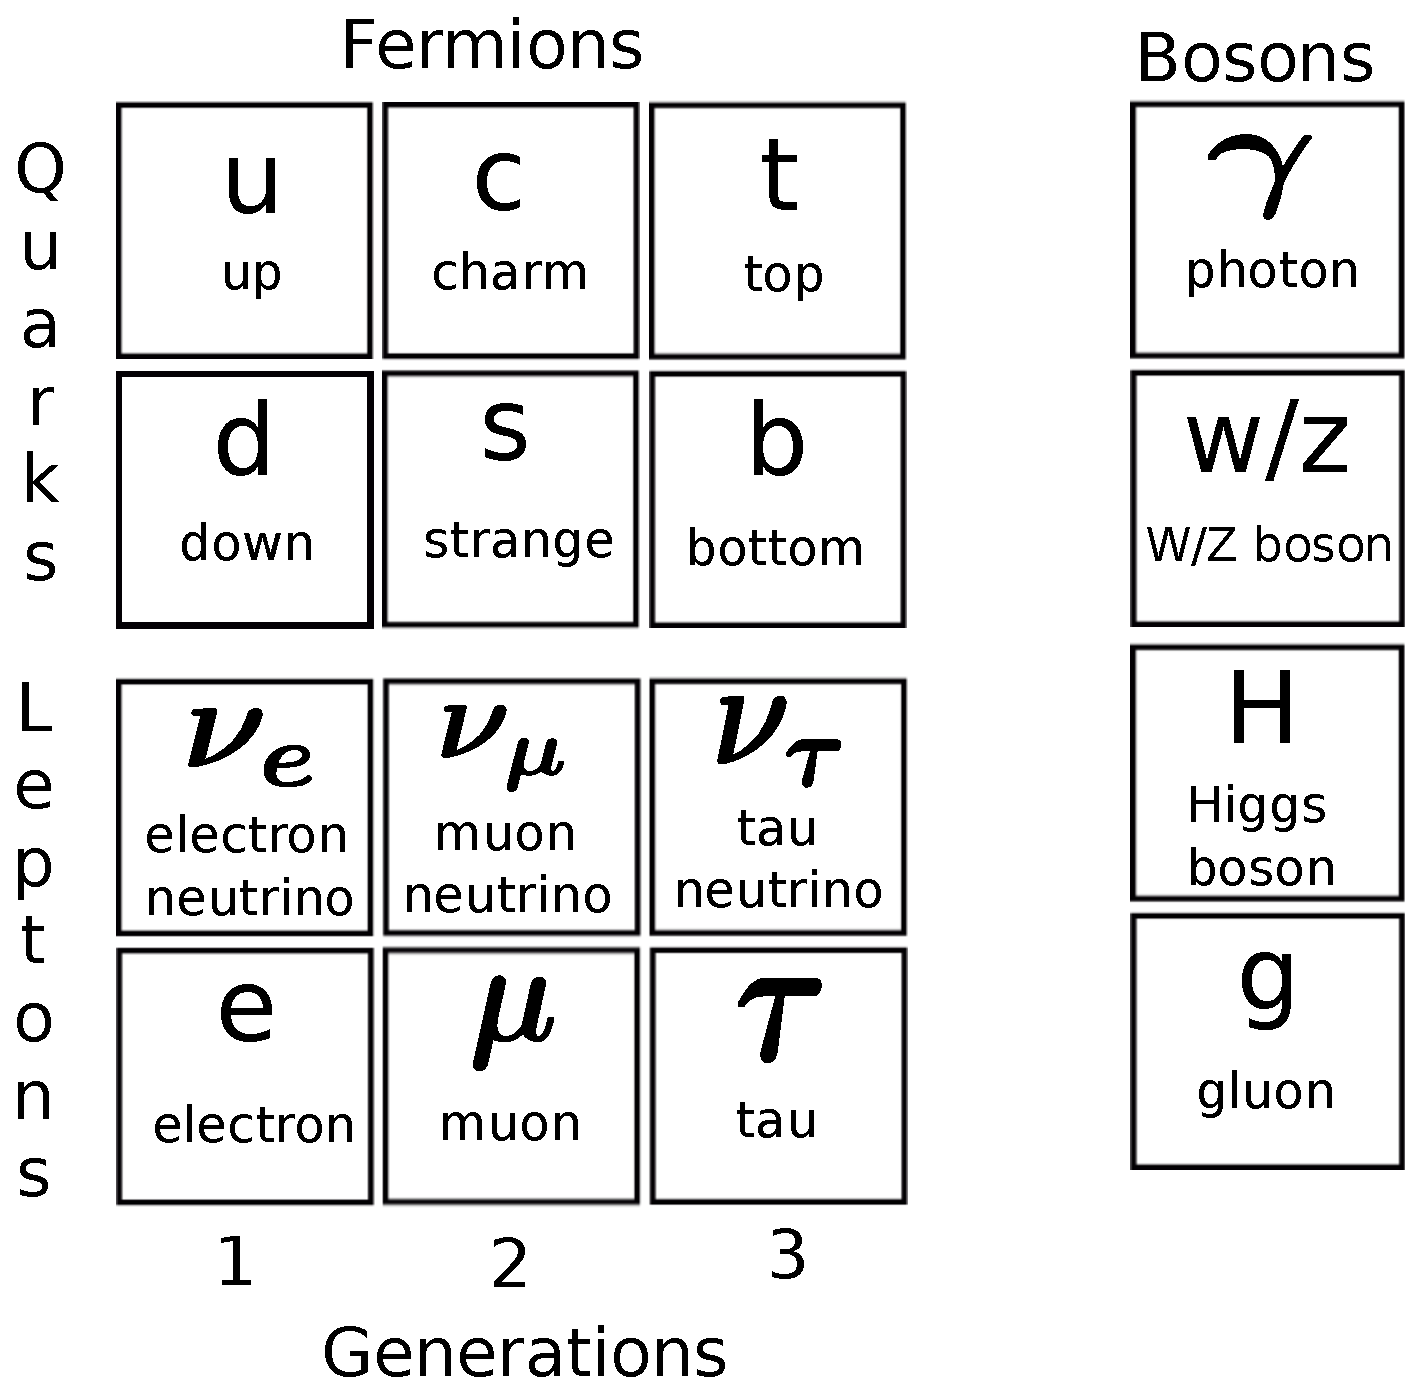
\includegraphics[width=0.6\textwidth]{figures/Theory/SM.eps}
\caption[The fundamental particles in the Standard Model]{
The fundamental particles in the Standard Model.
\label{Theory:SM}}
\end{figure}

